\documentclass[
	12pt,				% tamanho da fonte
	openany,			% capítulos começam em pág ímpar (insere página vazia caso preciso)
	oneside, 			% oneside - twoside
	a4paper,			% tamanho do papel.
	chapter=TITLE,		% títulos de capítulos convertidos em letras maiúsculas
	section=TITLE,		% títulos de seções convertidos em letras maiúsculas
	sumario=tradicional,	
	%subsection=TITLE,	% títulos de subseções convertidos em letras maiúsculas
	%subsubsection=TITLE,% títulos de subsubseções convertidos em letras maiúsculas
	english,			% idioma adicional para hifenização
	brazil,				% o último idioma é o principal do documento
	]{abntex2}

% ---------------------------------------------------------------------------
% Inclui os comandos do projeto
% ---------------------------------------------------------------------------
% -----------------------------------------------------------------------------
% Pacotes fundamentais
% -----------------------------------------------------------------------------
\usepackage{xcolor}
\newcommand\myworries[1]{\textcolor{red}{[#1]}}
\usepackage{lmodern}		% Usa a fonte Latin Modern (Serifada, tipo Times New Roman
%\usepackage{helvet}		% Usa a fonte Helvetica (Tipo Arial)
%\renewcommand{\familydefault}{\sfdefault} tira o serifado
\usepackage[T1]{fontenc}		% Selecao de codigos de fonte.
\usepackage[utf8]{inputenc}		% Codificacao do documento (conversão automática dos acentos)
\usepackage{indentfirst}		% Indenta o primeiro parágrafo de cada seção.
\usepackage{color}				% Controle das cores
\usepackage{tikz}				% Inclusão de gráficos
\usepackage{graphicx}			% Inclusão de gráficos
\usepackage{microtype} 			% para melhorias de justificação
% -----------------------------------------------------------------------------
% Pacotes adicionais, usados no anexo do modelo de folha de identificação
% -----------------------------------------------------------------------------
\usepackage{multicol}
\usepackage{multirow}
% -----------------------------------------------------------------------------
% Pacotes adicionais, usados apenas no âmbito do Modelo Canônico do abnteX2
% -----------------------------------------------------------------------------
\usepackage{lipsum}				% para geração de dummy text
% -----------------------------------------------------------------------------
% Pacotes de citações
% -----------------------------------------------------------------------------
\usepackage[brazilian,hyperpageref]{backref}	 % Paginas com as citações na bibliografia
\usepackage[alf,abnt-etal-list=3,abnt-etal-cite=3, abnt-emphasize=bf]{abntex2cite}	% Citações padrão ABNT
\usepackage{pdflscape}
\usepackage{footnote}
\usepackage{pdfpages}
\usepackage{caption}

% -----------------------------------------------------------------------------
% Pacotes adicionados por @leolleocomp
% -----------------------------------------------------------------------------
\usepackage{booktabs}
\usepackage{adjustbox}
\usepackage{subcaption}
\usepackage[labelfont=bf]{caption}
\usepackage{gensymb}
\usepackage{amsmath}
\usepackage{array}
% \usepackage{float}
\usepackage{xcolor,colortbl}
\usepackage{longtable}
\usepackage{scalefnt}
\usepackage{listings}			% inserir codigo fonte
\usepackage{morewrites} % necessário pois estamos screvendo muitos arquivos

% -----------------------------------------------------------------------------
% Pacotes adicionados por @Gabrielr2508
% -----------------------------------------------------------------------------
\usepackage{hyperref}

\usepackage{tocloft}
% -- permite a adição de células especiais em tabelas
\newcommand{\specialcell}[2][c]{%
  \begin{tabular}[#1]{@{}c@{}}#2\end{tabular}}

\newcounter{equationset}
\newcommand{\equationset}[1]{% \equationset{<caption>}
  \refstepcounter{equationset}% Step counter
  \noindent\makebox[\linewidth]{Equação ~\theequationset: #1}
 }

%-------------------------------------------------------------------------------
% Adequação dos títulos dos capitulos, seções, subseções às normas da Univasf
% Added by @Gabrielr2508
%-------------------------------------------------------------------------------
\renewcommand{\ABNTEXchapterfont}{\fontseries{b}}
\renewcommand{\ABNTEXchapterfontsize}{\normalsize}

\renewcommand{\ABNTEXsectionfont}{\fontseries{m}}
\renewcommand{\ABNTEXsectionfontsize}{\normalsize}

\renewcommand{\ABNTEXsubsectionfont}{\fontseries{b}}
\renewcommand{\ABNTEXsubsectionfontsize}{\normalsize}

\renewcommand{\ABNTEXsubsubsectionfont}{\fontseries{m}}
\renewcommand{\ABNTEXsubsubsectionfontsize}{\normalsize}

%-------------------------------------------------------------------------------
% CONFIGURAÇÕES DE PACOTES
% Configurações do pacote backref
%-------------------------------------------------------------------------------
% Usado sem a opção hyperpageref de backref
\renewcommand{\backrefpagesname}{Citado na(s) página(s):~}
% Texto padrão antes do número das páginas
\renewcommand{\backref}{}
% Define os textos da citação
\renewcommand*{\backrefalt}[4]{
	\ifcase #1 %
		%Nenhuma citação no texto.%
	\or
		Citado na página #2.%
	\else
		Citado #1 vezes nas páginas #2.%
	\fi}%

%-------------------------------------------------------------------------------
% Configurações de aparência do PDF final
%-------------------------------------------------------------------------------
% alterando o aspecto da cor azul
\definecolor{blue}{RGB}{41,5,195}

% informações do PDF
\makeatletter
\hypersetup{
     	%pagebackref=true,
		pdftitle={\@title},
		pdfauthor={\@author},
    	pdfsubject={\imprimirpreambulo},
	    pdfcreator={LaTeX with abnTeX2},
		pdfkeywords={abnt}{latex}{abntex}{abntex2}{relatório técnico},
		colorlinks=true,			% false: boxed links; true: colored links
    	linkcolor=black,				% color of internal links
    	citecolor=black,				% color of links to bibliography
    	filecolor=black,			% color of file links
		urlcolor=black,
		bookmarksdepth=4
}
\makeatother
% ---

% ---
% Espaçamentos entre linhas e parágrafos
% ---

% O tamanho do parágrafo é dado por:
\setlength{\parindent}{1.3cm}

% Controle do espaçamento entre um parágrafo e outro:
\setlength{\parskip}{0.2cm}  % tente também \onelineskip

%-------------------------------------------------------------------------------
% compila o indice
%-------------------------------------------------------------------------------
\makeindex
% ---

%-------------------------------------------------------------------------------
% Comando para inserir imagens de forma simples
%-------------------------------------------------------------------------------
\newcommand{\imagem}[4]
{%			\imagem{x.x}{nomeimg}{titulo}{fonte}
	\begin{figure}[!htb]
		\caption{\label{img:#2}#3}
		\begin{center}
			\includegraphics[scale=#1]{img/#2}
		\end{center}
        \legend{\textbf{Fonte:} #4}
	\end{figure}
}%

%-------------------------------------------------------------------------------
% Creio que esses comandos sejam para desenhar algo, aguardando explicações de @leolleocomp
%-------------------------------------------------------------------------------
\newcommand{\xx} {$\bigotimes$}
\newcommand{\oo} {$\bigcirc$}

%-------------------------------------------------------------------------------
% Biblioteca para códigos-fonte
%-------------------------------------------------------------------------------
\usepackage[newfloat=true]{minted}

%-------------------------------------------------------------------------------
% Caixas batutas - by @leolleocomp
%-------------------------------------------------------------------------------
\usepackage[most]{tcolorbox}
\tcbuselibrary{breakable}

\tcbuselibrary{minted}
\tcbset{listing engine=minted}

\definecolor{bg}{rgb}{0.95,0.95,0.95}

\SetupFloatingEnvironment{listing}{name=Código, listname=Lista de códigos}

%-------------------------------------------------------------------------------
% configuração do contador dos códigos-fonte - by @leolleocomp
% assim como as figuras, começa em 1
\newcounter{sourcecode}
%-------------------------------------------------------------------------------
%-------------------------------------------------------------------------------
% @leolleocomp
% stackoverflow code
% peguei da resposta abaixo
% https://stackoverflow.com/questions/24086366/change-latex-minted-listings-numbering-to-include-current-section?answertab=votes#tab-top
%-------------------------------------------------------------------------------
\makeatletter
\renewcommand*{\thelisting}{\thesourcecode}
\makeatother

%-------------------------------------------------------------------------------
% Peçam explicações a @leolleo
% WHO DID THIS?
%-------------------------------------------------------------------------------
\newcommand{\Ididthis}{
%	\legend{\textbf{Fonte:} O autor (\the\year).}
\legend{\textbf{Fonte:} O autor}
}

\newcommand{\Otherguydidthis}[1]{
	\legend{\textbf{Fonte:} \citeonline{#1}.}
}

%-------------------------------------------------------------------------------
% Comando para inserir códigos - by @leolleocomp
%-------------------------------------------------------------------------------
\newcommand{\sourcecode}[4]{
\begin{listing}[h]
	\refstepcounter{sourcecode}
	\caption{#1}
	\label{cmd:#2}
	\inputminted[linenos, bgcolor=bg, tabsize=4,breaklines]{#3}{codes/#4}
	\Ididthis
\end{listing}
}


% -----------------------------------------------------------------------------
% Pacotes adicionados por @ruanmed
% -----------------------------------------------------------------------------
\usepackage[binary-units=true]{siunitx}


%-------------------------------------------------------------------------------
% Comando para inserir códigos - by @ruanmed
%-------------------------------------------------------------------------------
\usepackage{caption}

\newenvironment{code}{\captionsetup{type=listing}}{}
\SetupFloatingEnvironment{listing}{name=Código}

\newcommand{\sourcecodenolist}[4]{
	\begin{code}
	    \refstepcounter{sourcecode}
        \captionof{listing}{#1 }
        \label{code:#2}
        \inputminted[linenos, bgcolor=bg, tabsize=4,breaklines]{#3}{codes/#4}
        \Wedidthis
    \end{code}
}

\newcommand{\sourcecodeinline}[2]{
	\mintinline[linenos, bgcolor=bg, tabsize=4,breaklines]{#1}{#2}
}


% CONFIGURACAO DO SUMARIO
%-------------------------------------------------------------------------------
% Modifica o espaçamento no sumário
% Nao ha espacos, exceto para as entradas de capitulos
\setlength{\cftbeforeparagraphskip}{0pt}
\setlength{\cftbeforesubsectionskip}{0pt}
\setlength{\cftbeforesectionskip}{0pt}
\setlength{\cftbeforesubsubsectionskip}{0pt}
\setlength{\cftbeforechapterskip}{\onelineskip}

% Alteração da indentação dos itens do sumário
\cftsetindents{chapter}{0pt}{42pt}
\cftsetindents{section}{0pt}{42pt}
\cftsetindents{subsection}{0pt}{42pt}
\cftsetindents{subsubsection}{0pt}{42pt}

% Modifica a formatacao dos textos

% Secao Primaria (Chapter): Caixa alta, Negrito, tamanho 12
\makeatletter
\settocpreprocessor{chapter}{%
  \let\tempf@rtoc\f@rtoc%
  \def\f@rtoc{%
  \texorpdfstring{\bfseries\MakeTextUppercase{\tempf@rtoc}}{\tempf@rtoc}}%
}
\makeatother

% Novo list of (listings) para QUADROS
% retirado de https://github.com/abntex/abntex2/wiki/HowToCriarNovoAmbienteListing

\newcommand{\quadroname}{Quadro}
\newcommand{\listofquadrosname}{Lista de quadros}

\newfloat[chapter]{quadro}{loq}{\quadroname}
\newlistof{listofquadros}{loq}{\listofquadrosname}
\newlistentry{quadro}{loq}{0}

% configurações para atender às regras da ABNT
\setfloatadjustment{quadro}{\centering}
\counterwithout{quadro}{chapter}
\renewcommand{\cftquadroname}{\quadroname\space}
\renewcommand*{\cftquadroaftersnum}{\hfill--\hfill}

% Configuração de posicionamento padrão:
\setfloatlocations{quadro}{hbtp}


% ---------------------------------------------------------------------------
% IDENTIFICAÇÃO
% ---------------------------------------------------------------------------
\titulo{ISSO AQUI DEU MUITO TRABALHO PARA SER FEITO}
\autor{FULANO DA SILVA}
\local{JUAZEIRO - BA}
\orientador{Prof. M. Sc. Ciclano Fulano de Tal}
%\coorientador{M. Sc. Osvaldo Campelo de Mello Vasconselos}
\instituicao{
UNIVERSIDADE FEDERAL DO VALE DO SÃO FRANCISCO
	\par
CURSO DE GRADUAÇÃO EM ENGENHARIA DE COMPUTAÇÃO}
\tipotrabalho{Trabalho de Conclusão de Curso}
\preambulo{Trabalho apresentado à Universidade Federal do Vale do São Francisco - Univasf, Campus Juazeiro, como requisito da obtenção do título de Bacharel em Engenharia de Computação.}


% -----------------------------------------------------------------------------
% CONFIGURACAO DO SUMARIO - by @Gabrielr2508
% Precisa estar aqui, por isso não foi para o commands.tex, não descobrimos o motivo, %caso saiba, por favor, faça um pull request! :D
% -----------------------------------------------------------------------------
% Secao primaria (Chapter) Caixa alta, Negrito, tamanho 12
\makeatletter
\renewcommand*{\l@chapter}[2]{%
  \l@chapapp{\uppercase{#1}}{#2}{\cftchaptername}}
\makeatother
% Secao secundaria (Section) Caixa baixa, Negrito, tamanho 12
\renewcommand{\cftsectionfont}{\uppercase} %ponha \rmfamily se quiser serifadas...

% Secao terciaria (Subsection) Caixa baixa, negrito, tamanho 12
\renewcommand{\cftsubsectionfont}{\bfseries}

% Secao quaternaria (Subsubsection) Caixa baixa, tamanho 12
\renewcommand{\cftsubsubsectionfont}{\normalfont}

% Seção quinaria (subsubsubsection) Caixa baixa, sem negrito, tamanho 12
\renewcommand{\cftparagraphfont}{\normalfont\itshape}

% -----------------------------------------------------------------------------
% Início do TCC 
% -----------------------------------------------------------------------------
\begin{document}

	\frenchspacing % Retira espaço extra obsoleto entre as frases.
	
	\pretextual
		%--------------------------------------------------------------------------------
% Constrói a capa com base na seção de identificação do main.tex
%--------------------------------------------------------------------------------
\begin{capa}
    \setlength{\belowcaptionskip}{0pt}
    \setlength{\abovecaptionskip}{0pt}
    \setlength{\intextsep}{-18pt}
        \begin{figure}[h]
    		\begin{center}
    		    
\includegraphics[scale=.5]{img/NEW_LOGO_UNIVASF.jpg}
    		\end{center}
    	\end{figure}

        %
\includegraphics[scale=0.6]{img/univasf.jpg}
        \center
    	{\ABNTEXchapterfont\large\imprimirinstituicao}

    	\vspace*{2cm}
    	    {\imprimirautor}
    	\vspace*{2cm}
        \begin{center}
    		\ABNTEXchapterfont\bfseries\large\imprimirtitulo
        \end{center}
    	\vfill

    	\ABNTEXchapterfont\bfseries\large\imprimirlocal\\
    	\the\year

    	\vspace*{1cm}
\end{capa}
%--------------------------------------------------------------------------------
% Constrói a folha de rosto com base na seção de identificação do main.tex
%--------------------------------------------------------------------------------
\begin{folhaderosto}
    \center
    	{\ABNTEXchapterfont\large\imprimirinstituicao}

		\vspace*{2cm}
    	    {\imprimirautor}
    	\vspace*{2cm}
		\vspace*{\fill}

		{\ABNTEXchapterfont\bfseries\large\imprimirtitulo}
		\vspace*{\fill}

		{\hspace{.45\textwidth}
		\begin{minipage}{.5\textwidth}
			\SingleSpacing
			\imprimirpreambulo \\ \\

			{\imprimirorientadorRotulo~\imprimirorientador\par}
			{\imprimircoorientadorRotulo~\imprimircoorientador\par}

		\end{minipage}%
		\vspace*{\fill}}%
		\vspace*{\fill}
			\ABNTEXchapterfont\bfseries\large\imprimirlocal\\
			\the\year
		\vspace*{1cm}
\end{folhaderosto}

%--------------------------------------------------------------------------------
% Constrói a ficha catalográfia com base na seção de identificação do main.tex
% Está comentado porque no final das contas a biblioteca do seu campus que gera a
% numeração, você pode adicionar os numeros aqui, ou anexar o pdf gerado por eles
% ao documento.
%--------------------------------------------------------------------------------
%\begin{fichacatalografica}
%	\vspace*{\fill}					% Posição vertical
%	\hrule							% Linha horizontal
%	\begin{center}					% Minipage Centralizado
%	\begin{minipage}[c]{12.5cm}		% Largura
%
%	\imprimirautor
%
%	\hspace{0.5cm} \imprimirtitulo  / \imprimirautor. --
%	\imprimirlocal, \the\year-
%
%	\hspace{0.5cm} xx p. : il. (algumas color.) ; 30 cm.\\
%
%	\hspace{0.5cm} \imprimirorientadorRotulo~\imprimirorientador\\
%
%	\hspace{0.5cm}
%	\parbox[t]{\textwidth}{\imprimirtipotrabalho~--~\imprimirinstituicao,
%	\the\year.}\\
%
%	\hspace{0.5cm}
%		1. Palavra-chave1.
%		2. Palavra-chave2.
%		I. Orientador.
%		II. Universidade xxx.
%		III. Faculdade de xxx.
%		IV. Título\\
%
%	\hspace{8.75cm} CDU 02:141:005.7\\
%
%	\end{minipage}
%	\end{center}
%	\hrule
%\end{fichacatalografica}

%--------------------------------------------------------------------------------
% Anexando a ficha catalogáfica e a folha de aprovação
%--------------------------------------------------------------------------------
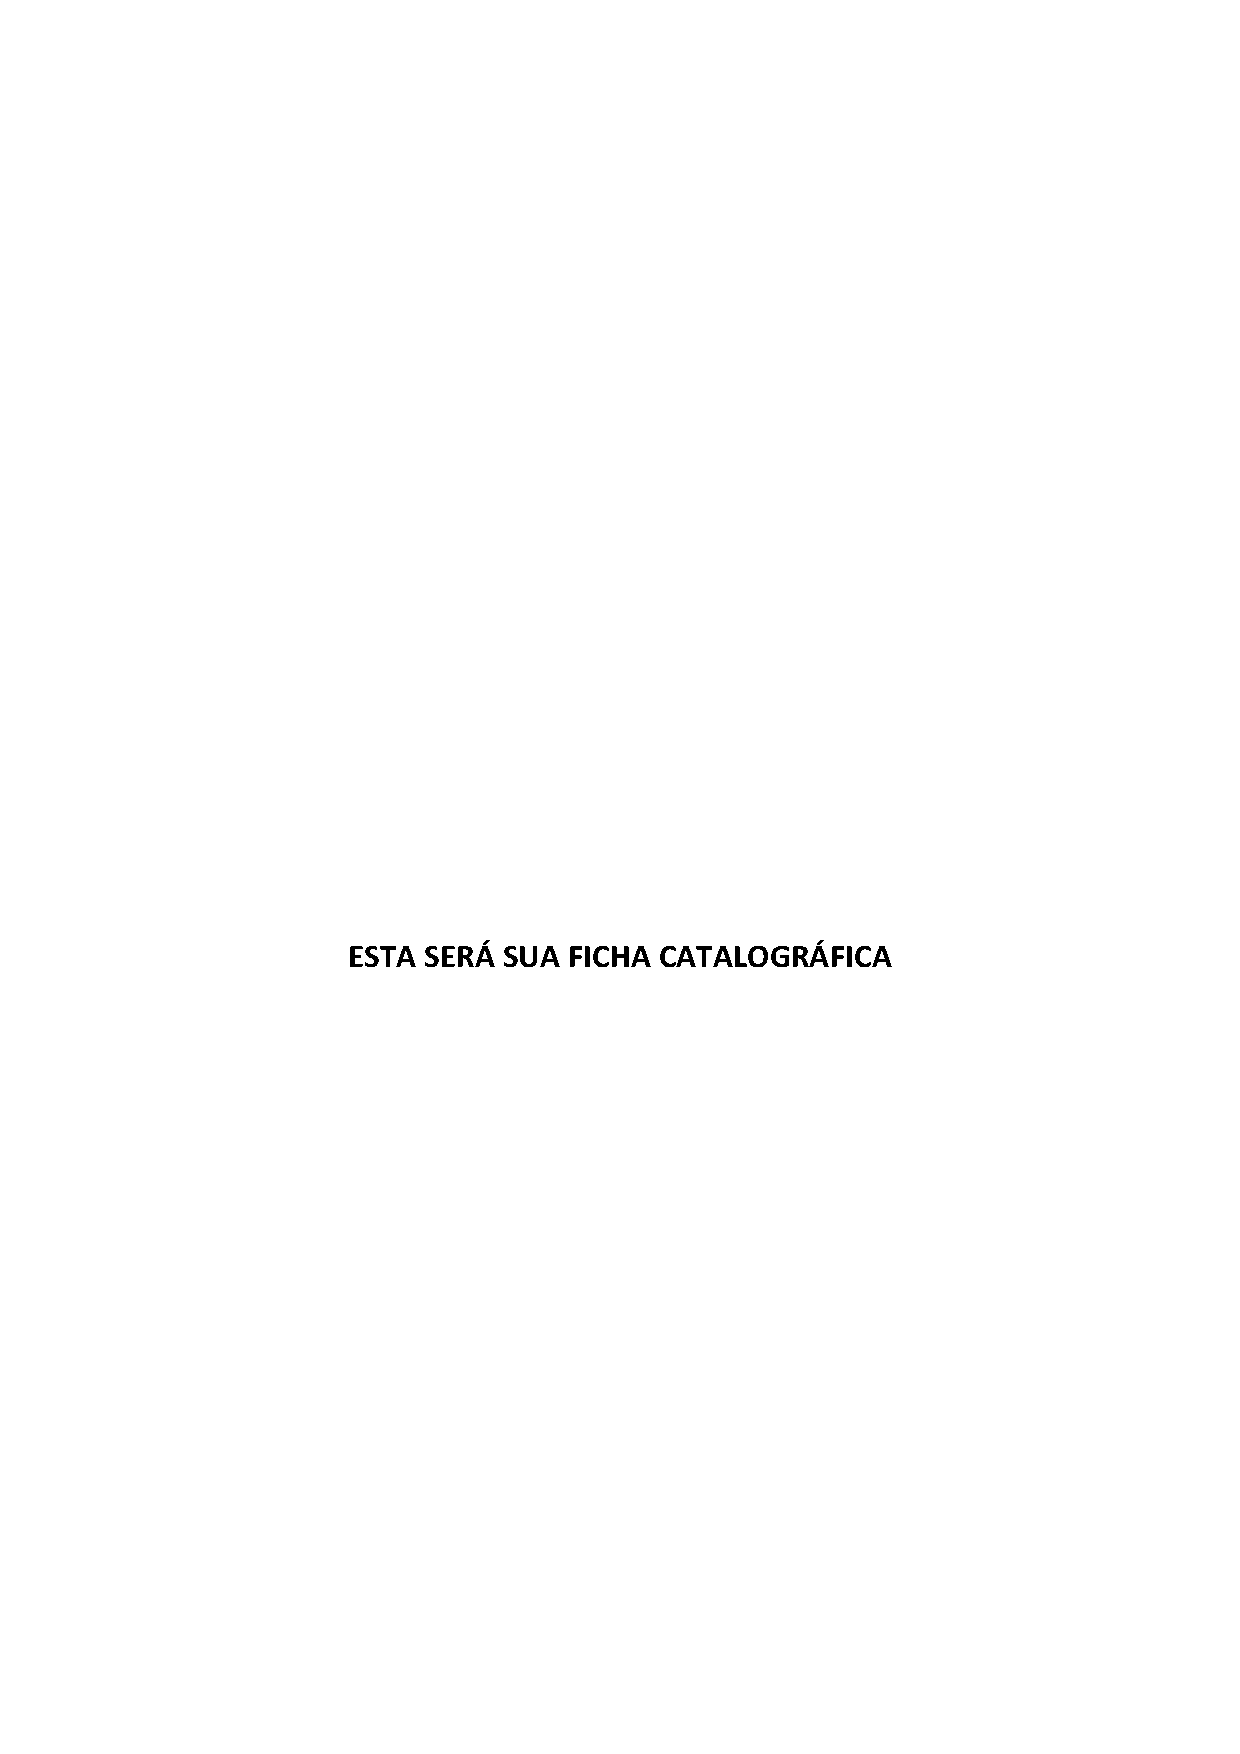
\includepdf[pages=-]{anexos/ficha.pdf}

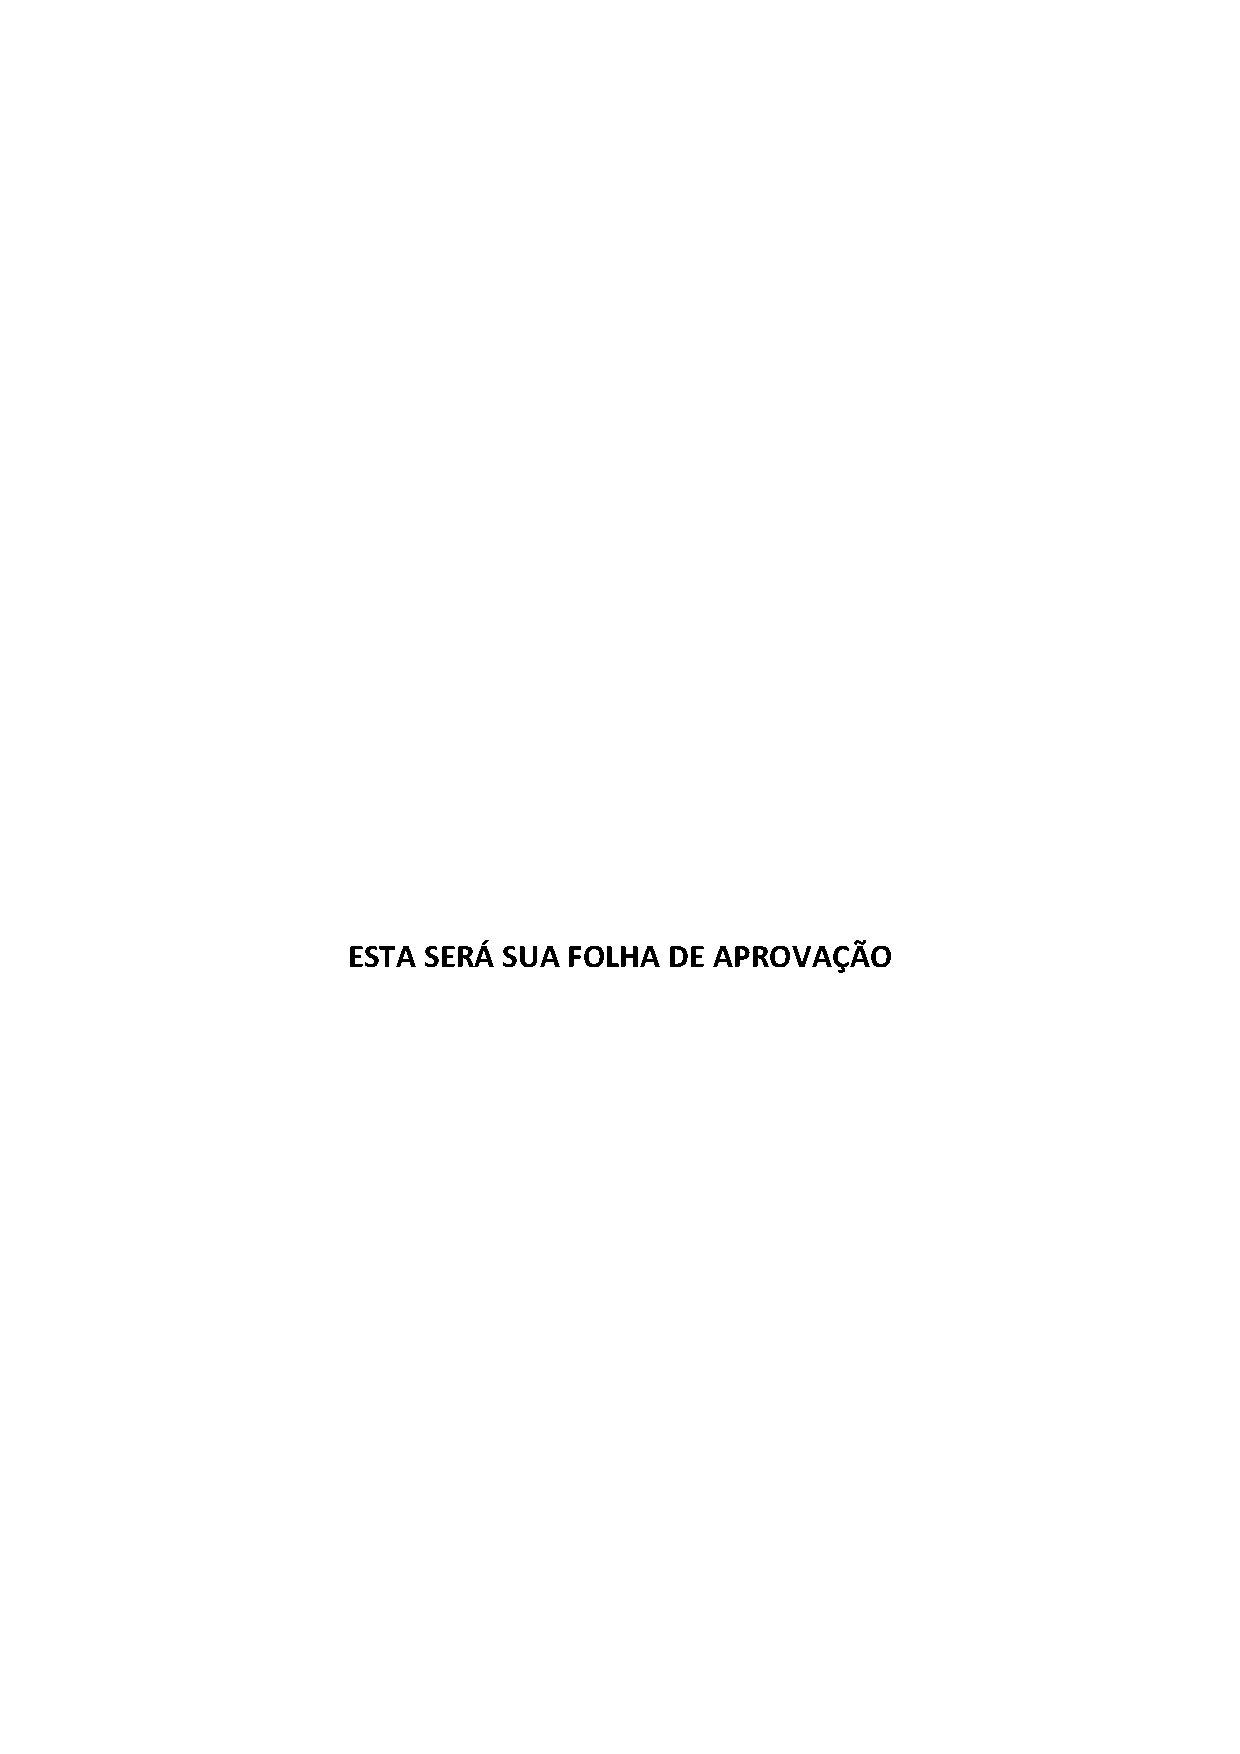
\includepdf[pages=-]{anexos/aprovacao.pdf}

\setlength{\ABNTEXsignwidth}{12cm}

%--------------------------------------------------------------------------------
% Está comentado pelo mesmo motivo da ficha catalográfica
%--------------------------------------------------------------------------------
%\begin{folhadeaprovacao}
%	\begin{center}
%	    {\ABNTEXchapterfont\bfseries\large\imprimirinstituicao}
%	    \vspace*{\fill}
%
%	    {\ABNTEXchapterfont\bfseries\large FOLHA DE APROVAÇÃO}
%	    \vspace*{\fill}
%
%	    {\ABNTEXchapterfont\bfseries\large\imprimirautor}
%
%	    \vspace*{\fill}\vspace*{\fill}
%	    {\ABNTEXchapterfont\bfseries\large\imprimirtitulo}
%	    \vspace*{\fill}
%
%	    {\hspace{.45\textwidth}
%		\begin{minipage}{.5\textwidth}
%			\SingleSpacing
%			\ABNTEXchapterfont\imprimirpreambulo \\ \\
%
%			{\ABNTEXchapterfont\imprimirorientadorRotulo~\imprimirorientador\par}
%			{\ABNTEXchapterfont\imprimircoorientadorRotulo~\imprimircoorientador\par}
%
%		\end{minipage}%
%	    \vspace*{\fill}}
%	\end{center}
%
%	\vspace*{\fill}
%
%	\begin{center}
%			 \ABNTEXchapterfont\large Aprovado em: \_\_\_\_ de \_\_\_\_ de 2017
%	\end{center}

%	\vspace*{\fill}

%	\begin{center}
%			 \ABNTEXchapterfont\bfseries\large Banca Examinadora
%	\end{center}
%
%   \ABNTEXchapterfont\assinatura{Fábio Nelson de Sousa Pereira, Mestre, Universidade Federal do Vale do São Francisco}
%	\ABNTEXchapterfont\assinatura{Jorge Luis Cavalcanti Ramos, Doutor, Universidade Federal do vale do São Francisco}
%  \ABNTEXchapterfont\assinatura{Ricardo Argenton Ramos, Doutor, Universidade Federal do Vale do São Francisco}
%	 \vspace*{\fill}


%\end{folhadeaprovacao}

%--------------------------------------------------------------------------------
% Insere a epígrafe
%--------------------------------------------------------------------------------
\newpage
\vspace*{\fill}
\begin{flushright}
		\textit{Lorem Ipsum...}
\end{flushright}

%--------------------------------------------------------------------------------
% Seção de agradecimentos
%--------------------------------------------------------------------------------
\begin{agradecimentos}

\lipsum[2-4]

\end{agradecimentos}

%--------------------------------------------------------------------------------
% Insere a segunda epígrafe
%--------------------------------------------------------------------------------
\begin{epigrafe}
    \vspace*{\fill}
	\begin{flushright}
		Se pude enxergar a tão grande distância, foi subindo nos ombros de gigantes.\\
		 \vspace{\baselineskip}
		\textbf{Isaac Newton}\\
		\textbf{Carta à Robert Hooke, 1676}
	\end{flushright}
\end{epigrafe}



%--------------------------------------------------------------------------------
% Seção de resumos
%--------------------------------------------------------------------------------
% resumo em português
\setlength{\absparsep}{18pt} % ajusta o espaçamento dos parágrafos do resumo
\begin{resumo}

\lipsum[1-2]

 \textbf{Palavras-chave}: \textit{Palavra em inglês 1, Palavra em inglês 2, Palavra em inglês 3, Palavra em inglês 4}, Palavra 5.

\end{resumo}

%---------------------------------------------------------------------------------
% resumo em inglês
\begin{resumo}[Abstract]
\begin{otherlanguage*}{english}

\lipsum[3-4]

	\vspace{\onelineskip}

	\noindent
	\textbf{Key-words}: \textit{Palavra em inglês 1, Palavra em inglês 2, Palavra em inglês 3, Palavra em inglês 4, Palavra em inglês 4}.

\end{otherlanguage*}
\end{resumo}


%---------------------------------------------------------------------------------
% Insere lista de ilustrações
%---------------------------------------------------------------------------------
\begin{KeepFromToc} % Este comando evita que todas as seções dentro dele de apareçam no sumário
\pdfbookmark[0]{\listfigurename}{lof}
\listoffigures
%\addcontentsline{toc}{chapter}{Lista de Figuras}
\cleardoublepage


%---------------------------------------------------------------------------------
% Insere lista de tabelas
%---------------------------------------------------------------------------------
\pdfbookmark[0]{\listtablename}{lot}
\listoftables
\cleardoublepage

%---------------------------------------------------------------------------------
% Insere lista de quadros
%---------------------------------------------------------------------------------
\pdfbookmark[0]{\listofquadrosname}{loq}
\listofquadros*
\cleardoublepage

%---------------------------------------------------------------------------------
% Ajusta lista de código - alterar de figures para códigos - by @Gabrielr2508
%---------------------------------------------------------------------------------
\makeatletter
\let\l@listing\l@figure
\def\newfloat@listoflisting@hook{\let\figurename\listingname}
\makeatother

%---------------------------------------------------------------------------------
% Insere lista de códigos - by @leolleocomp
%---------------------------------------------------------------------------------
\listoflistings

\end{KeepFromToc}

%---------------------------------------------------------------------------------
% Insere lista de abreviaturas e siglas
%---------------------------------------------------------------------------------
\begin{siglas}
	\item[LI]       Lorem Ipsum
    \item[LII]		Lorem Ipsum Ipsum

\end{siglas}

%---------------------------------------------------------------------------------
% Insere o sumario
%---------------------------------------------------------------------------------
\pdfbookmark[0]{\contentsname}{toc}
\tableofcontents*
\cleardoublepage




	\textual
		\pagestyle{simple}
		%--------------------------------------------------------------------------------------
% Este arquivo contém a sua introdução, objetivos e organização do trabalho
%--------------------------------------------------------------------------------------
\chapter{Introdução}

\lipsum[5-10]

Colocar citações longas entre \textbackslash begin\{citacao\} e \textbackslash end\{citacao\}, exemplo: 

\begin{citacao}
``\lipsum[1]''

\cite{REFERENCIA}
\end{citacao}

\section{Justificativa}

\lipsum[1]


\section{Objetivos gerais}

\lipsum[1]

\section{Objetivos específicos}

\begin{itemize}
	\item blablablabla;
    \item blablablabla;
    \item blablablabla.
\end{itemize}

\section{Organização do trabalho}

\lipsum[10-12]

		%--------------------------------------------------------------------------------------
% Este arquivo contém a sua funtamentação teórica
%--------------------------------------------------------------------------------------
\chapter{Referencial teórico}

\section{Seção de exemplo 1 - Como fazer citações}

Existem vários tipos de citações...


\section{Seção de exemplo 2 - Como inserir figuras}

Neste trabalho iremos exemplificar duas formas de se inserir figuras no Latex. O primeiro método insere, no documento, uma figura simples por meio do comando:

\textbackslash imagem\{ Escala \}\{ Arquivo sem extensão \}\{ Descrição \}\{ Fonte \}

\textbf{Obs.:} A fonte pode ser uma citação do tipo  \textbackslash citeonline\{\}.

A figura \ref{img:placeholder} é um exemplo deste método.

%--------------------------------------------------------------------------------------
% Esse é um exemplo de figura simples
%--------------------------------------------------------------------------------------
\imagem{0.15}{placeholder}{Uma figura simples}{O autor}

A figura \ref{img:figura1} é um exemplo do outro tipo de figura abordada aqui, chamada de figura composta. Esta figura é composta de outras subfiguras.
%--------------------------------------------------------------------------------------
% Esse é um exemplo de figura composta de outras subfiguras
%--------------------------------------------------------------------------------------
\begin{figure}[!htb]
\centering
    \caption{\label{img:figura1} Exemplo de figura composta}
    \subcaptionbox{\label{img:subfigura1} Subfigura 1}{
\includegraphics[scale=.1]{img/placeholder}}\qquad
    \subcaptionbox{\label{img:subfigura2} Subfigura 2}{
\includegraphics[scale=.1]{img/placeholder}}
    \vspace{1.5em}
    \legend{\textbf{Fonte:} \citeonline{SUA-REFERENCIA}}
\label{fig:dag}
\end{figure}

%\begin{figure}[!htb]
%\centering
%    \caption{\label{img:telas} Telas da aplicação cliente}
%    \subcaptionbox{\label{img:inicial} Abertura}{\includegraphics[scale=.12]{img/APP/inicial}}\qquad
%    \subcaptionbox{\label{img:login} \textit{Login}}{\includegraphics[scale=.12]{img/APP/login}}\qquad
%    \subcaptionbox{\label{img:cadastro} Cadastro}{\includegraphics[scale=.12]{img/APP/cadastro}}\qquad
%    \subcaptionbox{\label{img:hist-rel}Sobre}{\includegraphics[scale=.12]{img/APP/sobre}}\\
%    \vspace{1.5em}
%    \subcaptionbox{\label{img:dados_atuais}Dados atuais}{\includegraphics[scale=.15]{img/APP/atual}}\qquad
%    \subcaptionbox{\label{img:hist-time}Seleção de período}{\includegraphics[scale=.15]{img/APP/periodo}}\qquad
%    \subcaptionbox{\label{img:hist-rel}Exibir histórico}{\includegraphics[scale=.15]{img/APP/historico}}\\
%    \vspace{2.5em}
%    \legend{\textbf{Fonte:} O Autor}
%\label{fig:dag}
%\end{figure}

Para referenciar uma figura deve ser usada comando \textbackslash ref\{img:<label ou nome do arquivo>\}, como exemplo, estamos referenciando a figura \ref{img:placeholder}. Isso vale tanto para figuras simples quanto para as compostas, como por exemplo as figuras \ref{img:subfigura1} e \ref{img:subfigura2}. Ao inserir uma figura, ela é automaticamente identificada e incluída no elemento pré-textual da lista de figuras.




\section{Seção de exemplo 3 - Sobre tabelas}

As tabelas em Latex são deveras capciosas, por isso não serão abordadas em sua completude neste documento.

Há um site que possui uma ferramenta interessante para ser utilizada na construção tabelas em Latex.

\centerline{\href{https://www.tablesgenerator.com/}{ O Tables Generator } <-- Isto é um \textit{link} :D}

Contudo, busquem entendimento sobre o assunto, pois tabelas são elementos textuais importantes e enriquecem muito o texto, quando bem construídas.

A tabela \ref{tab:crossplatform} é um exemplo de como uma tabela pode ser construída, assim como a tabela do anexo \ref{anex:anexo1}.

\begin{table}[!htb]
	\centering
	\caption{\label{tab:crossplatform} Tipos de aplicações e abordagens preferenciais.}
	\begin{adjustbox}{max width=\textwidth}
		\begin{tabular}{@{} p{5cm} |c|c|c| @{}}
		\toprule
		\textbf{Código da Aplicação} & \textbf{Web} & \textbf{Híbrida} & \textbf{Interpretada / Compilação Cruzada} \\ \hline

		\textbf{Aplicações baseadas em dados providos por um servidor} &
			3 & 2 & 1
		\\ \hline

		\textbf{Aplicações independentes} & 1 & 2 & 3\\ \hline

		\textbf{Aplicações baseadas em sensores e processamento de dados no dispositivo} & 1 & 2 & 3\\ \hline

		\textbf{Aplicações baseadas em sensores e processamento de dados no servidor} & 1 & 3 & 2\\ \hline

		\textbf{Aplicações Cliente-Servidor} & 1 & 3 & 2 \\ \bottomrule
	\end{tabular}
	\end{adjustbox}
	\legend{\textbf{Fonte:} \citeonline{raj2012study} (Traduzido)}
\end{table}

Também é possível criar quadros, que são ligeiramente diferente de tabelas. Acompanhe o exemplo no Quadro \ref{qua:confusionmatrix}

\begin{quadro}
	\centering
	\caption{\label{qua:confusionmatrix}Exemplo de matriz de confusão}
	\begin{tabular}{ll|c|c|}
		\cline{3-4}
		\multicolumn{1}{c}{\textbf{}} & \multicolumn{1}{c|}{\textbf{}} & \multicolumn{2}{l|}{\textbf{Classe prevista}} \\ \cline{3-4}
		 & \multicolumn{1}{c|}{\textbf{}} & Classe = 1 & Classe = 0 \\ \hline
		\multicolumn{1}{|l|}{\multirow{2}{*}{\textbf{Classe real}}} & Classe = 1 & $f_{11}$ & $f_{10}$ \\ \cline{2-4}
		\multicolumn{1}{|l|}{} & Classe = 0 & $f_{01}$ & $f_{00}$ \\ \hline
	\end{tabular}
	\Ididthis
\end{quadro}


\begin{quadro}
	\caption{\label{qua:cron}Cronograma}
	\center
	\begin{tabular}{|c|c|c|c|c|c|}
	\hline
	\multicolumn{1}{|l|}{Atividade} & \multicolumn{1}{l|}{Set/19} & \multicolumn{1}{l|}{Out/19} & \multicolumn{1}{l|}{Nov/19} & \multicolumn{1}{l|}{Dez/19} & \multicolumn{1}{l|}{Jan/20} \\ \hline
	1                               & x                           &                             &                             &                             &                             \\ \hline
	2                               &                             & x                           &                             &                             &                             \\ \hline
	3                               &                             & x                           &                             &                             &                             \\ \hline
	4                               &                             &                             & x                           & x                           &                             \\ \hline
	5                               &                             & x                           & x                           & x                           &                             \\ \hline
	6                               &                             &                             &                             &                             & x                           \\ \hline
	
	\end{tabular}
	\legend{\textbf{Fonte:} Elaborado pela autora (2019)}
	\end{quadro}

\section{Subseção de exemplo 4 - Seções}

		%--------------------------------------------------------------------------------------
% Este arquivo contém a sua metodologia
%--------------------------------------------------------------------------------------
\chapter{Materiais e Métodos} \label{ch:MM} %Uma label é como você referencia uma seção no texto com a tag \ref{}


\section{Seção de exemplo 1} 



\subsection{Subseção de exemplo 1 - Referenciando seções} \label{subsec:subsec1}






%--------------------------------------------------------------------------------------
% Insere a seção de cronograma
% Está comentada porque só é necessária no TCC I
%--------------------------------------------------------------------------------------

%\section{Cronograma} \label{sec:crono}

%A tabela \ref{tab:cronograma} mostra o cronograma de atividades a serem executadas para o TCC II, com base no calendário de 201X.Y da UNIVASF.

%\newpage
%\begin{table}[!thb]
%	%\huge
%    \centering
%    \caption{\label{tab:cronograma} Cronograma das atividades previstas para o TCC II}
%%    \begin{adjustbox}{max width=\textwidth}
%    \begin{tabular}{p{6.5cm}|c|c|c|c|c|c}
%    \toprule
%    \textbf{Atividade}                      & Nov & Dez & Jan & Fev & Mar & Abr \\ \hline
%    Implementar o banco de dados              & X    & X     &       &        &          &          \\ \hline
%    Desenvolver a API HTTP RESTful                      &   X   & X     &       &        &          &          \\ \hline
%    Implementar o serviço de captura de dados        &      &      & X     &   X     &          &          \\ \hline
%    Desenvolver a aplicação \textit{Web/mobile} para exibição dos dados         &      &      & X     &   X     &     X     &          \\ \hline
 %   Teste do sistema            &      &       &       &        & X        &          %\\ \hline
 %   Escrita do TCC II                       &   X   & X     & X     & X      & X        & X        \\ \hline
%   Defesa do TCC II                        &      &       &       &        &          & X       \\
%    \bottomrule
 %   \end{tabular}
 %   \end{adjustbox}
%    \legend{\textbf{Fonte:} O autor.}
%\end{table}


		\chapter{Resultados} \label{ch:RD}



\section{Seção de exemplo 1 - Códigos} \label{sec:resex1}

\subsection{Subseção de exemplo 1 - Inserindo trechos de códigos}
 
O nosso querido Leonardo Cavalcante providenciou um comando que deixa nossos trechos de códigos bonitinhos e gera um elemento pré-textual de Lista de Códigos. 

Os códigos são adicionados através do comando seguinte:

\textbackslash sourcecode\{ Descrição \}\{Label\}\{Linguagem\}\{Arquivo com extensão\}

Um exemplo pode ser visto no código \ref{cmd:cron} abaixo.

\sourcecode{Configuração do intervalo de execução no Script Agendador}{cron}{javascript}{cron.js}


\section{Seção de exemplo 2 - Listas} \label{sec:resex2}

\subsection{Subseção de exemplo 2 - Lista de itens} 

Existem alguns tipos de listas no Latex, iremos exemplificar a lista sem numeração (seção \ref{subsubsec:itemize}), a lista enumerada (seção \ref{subsubsec:enumerate}) e a lista mista (seção \ref{subsubsec:mista}). As listas podem ser encadeadas de diversas maneiras,
de acordo com a necessidade do autor.

\subsubsection{Subsubseção de exemplo 1 - Lista sem numeração} \label{subsubsec:itemize}

Este é um exemplo de lista sem numeração.

\begin{itemize}
	\item \textbf{Cadastrar usuário}

		\begin{itemize}
    		\item Atores
		    	\begin{itemize}
    		    	\item Usuário
		    	\end{itemize}

	    	\item Fluxo de eventos primário
			    \begin{itemize}
	    		    \item o usuário deve se cadastrar informando seu nome, \textit{e-mail} e senha;
		        	\item a API armazena os dados do usuário;
		    	    \item o usuário é liberado para realizar o \textit{login}.
			    \end{itemize}

    		\item Fluxo alternativo
			    \begin{itemize}
		    	   \item o usuário desiste de se cadastrar e cancela o caso de uso clicando no botão voltar.
	    		\end{itemize}

		\end{itemize}
	
\end{itemize}

\subsubsection{Subsubseção de exemplo 2 - Lista enumerada} \label{subsubsec:enumerate}

Este é um exemplo de lista enumerada.

\begin{enumerate}
	\item O Usuário deseja ver o histórico das variáveis climáticas, então através da interface de usuário escolhe o período ao qual o histórico se refere;
	\item A aplicação solicita à API através de uma requisição HTTP contendo o momento de início e o momento do fim do período em seus parâmetros;     			\item A API recebe a solicitação e se comunica com a base de dados, então requere as informações quem possuem a data de leitura no intervalo escolhido;
	\item A base de dados retorna os dados em formato Json para a API;
	\item A API responde à requisição retornando os dados, também em formato Json, para a aplicação cliente;
	\item A aplicação cliente renderiza os gráficos utilizando o conjunto de dados obtidos.
\end{enumerate}

\subsubsection{Subsubseção de exemplo 3 - Lista mista} \label{subsubsec:mista}

Este é um exemplo de lista mista.

\begin{itemize}
	\item \textbf{Cadastrar usuário}

		\begin{itemize}
    		\item Atores
		    	\begin{itemize}
    		    	\item Usuário
		    	\end{itemize}

	    	\item Fluxo de eventos primário
			    \begin{enumerate}
	    		    \item o usuário deve se cadastrar informando seu nome, \textit{e-mail} e senha;
		        	\item a API armazena os dados do usuário;
		    	    \item o usuário é liberado para realizar o \textit{login}.
			    \end{enumerate}

    		\item Fluxo alternativo
			    \begin{itemize}
		    	   \item o usuário desiste de se cadastrar e cancela o caso de uso clicando no botão voltar.
	    		\end{itemize}

		\end{itemize}

	\item \textbf{Visualizar dados atuais}

		\begin{itemize}
		    \item Atores
	    		\begin{itemize}
		    	    \item Usuário
			    \end{itemize}
    
	    	\item Pré-condições
			    \begin{itemize}
		     	   \item o usuário deve estar autenticado
			    \end{itemize}

	    	\item Fluxo de eventos primário
			    \begin{enumerate}
		    	    \item o usuário deve efetuar o \textit{login} informando o \textit{e-mail} e a senha;
	    		    \item caso o usuário não seja autenticado, o sistema informa a respeito de credenciais inválidas e encerra o caso de uso;
		    	    \item a API autentica o usuário;
    			    \item o usuário é liberado para visualizar os dados atuais dos sensores da estação;
		        	\item após a visualização o usuário pode finalizar o caso de uso ou efetuar uma nova consulta se desejar.
			    \end{enumerate}

    		\item Fluxo alternativo
			    \begin{itemize}
    			   \item o usuário desiste de visualizar os dados atuais e cancela o caso de uso clicando no botão voltar.
			    \end{itemize}

		\end{itemize}

	\item \textbf{Visualizar histórico}

		\begin{itemize}
		    \item Atores
	    		\begin{itemize}
		    	    \item Usuário
	    		\end{itemize}

	    	\item Pré-condições
    			\begin{itemize}
			        \item o usuário deve estar autenticado
			    \end{itemize}

		    \item Fluxo de eventos primário
			    \begin{enumerate}
			        \item o usuário deve efetuar o \textit{login} informando o \textit{e-mail} e a senha;
			        \item caso o usuário não seja autenticado, o sistema informa a respeito de credenciais inválidas e encerra o caso de uso;
			        \item a API autentica o usuário;
			        \item o usuário é liberado para escolher qual período cujo histórico será exibido;
			        \item o usuário seleciona as variáveis a serem exibidas no gráficos de linhas;
			        \item após a visualização do histórico o usuário pode finalizar o caso de uso se desejar.
			    \end{enumerate}

		    \item Fluxo alternativo
			    \begin{enumerate}
			        \item após a escolha do período de exibição do histórico o usuário pode voltar para a tela anterior e escolher um novo período;
			        \item o histórico é exibido para o usuário;
			        \item após a visualização do histórico o usuário pode finalizar o caso de uso ou efetuar uma nova consulta se desejar.
			    \end{enumerate}

		    \item Fluxo alternativo
			    \begin{enumerate}
			        \item o usuário desiste de visualizar o histórico e cancela o caso de uso clicando no botão voltar.
			    \end{enumerate}
		\end{itemize}
\end{itemize}
		%--------------------------------------------------------------------------------------
% Este arquivo contém a sua conclusão
%--------------------------------------------------------------------------------------
\chapter{Considerações Finais e Trabalhos Futuros}

\lipsum[1-2]
 
\section{Trabalhos futuros}

\lipsum[55]

	\postextual
		\bibliography{tex/references}
		\begin{anexosenv}
\chapter{Comandos seriais da estação meteorológica \textit{Vantage Vue™}} \label{anex:anexo1}

\begin{center}
\scalefont{0.85}
\begin{longtable}{ll}
\caption{Comandos seriais suportados pela estação meteorológica \textit{Vantage Vue™}}\\
\hline
\multicolumn{1}{c}{\textbf{Instrução}} & \multicolumn{1}{c}{\textbf{Descrição}} \\ \hline
\endfirsthead

\multicolumn{2}{c}%
{{\bfseries \tablename\ \thetable{} -- Continuação da página anterior}} \\

\hline
\multicolumn{1}{c}{\textbf{Instrução}} & \multicolumn{1}{c}{\textbf{Descrição}} \\ \hline
\endhead

\multicolumn{2}{r}{{Continua na próxima página}} \\
\endfoot

\endlastfoot

\multicolumn{2}{c}{\cellcolor{gray!25}\textbf{Comandos de teste}}                                                   		 \\ \hline
\textbf{TESTE}                            & Envia a \textit{string} "TEST\textbackslash n" de volta  \\ \hline
\textbf{WRD}                        & Responde com o tipo de estação meteorológica \\ \hline
\textbf{RXCHECK}                        & Responde com o diagnóstico do Console \\ \hline
\textbf{RXTEST}                       & Muda a tela do console de \textit{"Receiving from"} para tela de dados atuais                                                        \\ \hline
\textbf{VER}                           & Responde com a data do \textit{firmware}                                                             \\ \hline
\textbf{RECEIVERS}                    & Responde com a lista das estações que o console "enxerga" \\ \hline
\textbf{NVER}                       & Responde com a versão do \textit{firmware}                                                             \\ \hline
\multicolumn{2}{c}{\cellcolor{gray!25}\textbf{Comandos de dados atuais}}                                             \\ \hline
\textbf{LOOP}                     & Responde com a quantidade de pacotes especificada a cada 2s        \\ \hline
\textbf{LPS}                & Responde a cada 2s com a quantidade de pacotes diferentes especificada          \\ \hline
\textbf{HILOWS}                & Responde com todo os dados de \textit{high/low}                 \\ \hline
\textbf{PUTRAIN}                      & Seta a quantidade anual de precipitação \\ \hline
\textbf{PUTET}                 & Seta a quantidade anual de evapotranspiração        \\ \hline
\multicolumn{2}{c}{\cellcolor{gray!25}\textbf{Comandos de \textit{download}}}                                     		 \\ \hline
\textbf{DMP}                 & Faz o \textit{download} de todo o arquivo de memória \\ \hline
\textbf{DMAFT}                   & Faz o \textit{download} de todo o arquivo de memória após a data especificada \\ \hline
\multicolumn{2}{c}{\cellcolor{gray!25}\textbf{Comandos da EEPROM}}                                     		 \\ \hline
\textbf{GETEE}                 & Lê toda a memória EEPROM \\ \hline
\textbf{EEWR}                   & Escreve um \textit{byte} de dados à partir do endereço especificado                                   \\ \hline
\textbf{EERD}                   & Lê a quantidade de dados especificada iniciando no endereço especificado                                   \\ \hline
\textbf{EEBWR}                   & Escreve os dados na EEPROM                                    \\ \hline
\textbf{EEBRD}                   & Lê os dados da EEPROM \\ \hline
\multicolumn{2}{c}{\cellcolor{gray!25}\textbf{Comandos de calibração}}                                     		 \\ \hline
\textbf{CALED}                 & Envia os dados da temperatura e umidade corrente para atribuir à calibração \\ \hline
\textbf{CALFIX}                   & Atualiza o \textit{display} quando os números de calibração mudam\\ \hline
\textbf{BAR}                   & Seta os valores da elevação e o \textit{offset} do barômetro quando a localização é alterada                                   \\ \hline
\textbf{BARDATA}                   & Mostra os valores atuais da calibração do barômetro                                   \\ \hline \\
\multicolumn{2}{c}{\cellcolor{gray!25}\textbf{Comandos de limpeza}}                                     		 \\ \hline
\textbf{CLRLOG}                 & Limpa todo o arquivo de dados                                                       \\ \hline
\textbf{CLRALM}                   & Limpa todos os limiares dos alarmes                                   \\ \hline
\textbf{CLRCAL}                   & Limpa todos os \textit{offsets} da calibração da temperatura e da umidade \\ \hline
\textbf{CLRGRA}                   & Limpa o gráfico do console \\ \hline
\textbf{CLRVAR}                   & Limpa o valor da precipitação ou da evapotranspiração \\ \hline
\textbf{CLRHIGHS}                   & Limpa todos os valores de pico diários, mensais ou anuais                                   \\ \hline
\textbf{CLRLOWS}                   & Limpa todos os valores de mínimos diários, mensais ou anuais \\ \hline
\textbf{CLRBITS}                   & Limpa os \textit{bits} de alarme ativos                                  \\ \hline
\textbf{CLRDATA}                   & Limpa todos os dados atuais                                   \\ \hline
\multicolumn{2}{c}{\cellcolor{gray!25}\textbf{Comandos de configuração}}                                     		 \\ \hline
\textbf{BAUD}                 & Atribui o valor do \textit{baudrate} do console                                                       \\ \hline
\textbf{SETTIME}                   & Define a data e a hora do console                                   \\ \hline
\textbf{GAIN}                   & Define o ganho do receptor de rádio                                   \\ \hline
\textbf{GETTIME}                   & Retorna a hora e a data atual do console                                   \\ \hline
\textbf{SETPER}                   & Define o intervalo de arquivamento                                   \\ \hline
\textbf{STOP}                   & Desabilita a criação dos registros                                   \\ \hline
\textbf{START}                   & Habilita a criação dos arquivos \\ \hline
\textbf{NEWSETUP}                   & Reinicia o console após alguma configuração nova                                  \\ \hline
\textbf{LAMPS}                   & Liga ou desliga as lâmpadas do console \\ \hline

%\label{tab:6}
\end{longtable}
\fonte{\citeonline{VSPDOC} (Traduzido).}
\end{center}


\end{anexosenv}


\end{document}
